\begin{enumerate}[label=\thesubsection.\arabic*,ref=\thesubsection.\theenumi]
\item Find the slope of the tangent to the curve $y = \frac{x-1}{x-2}$, $x \neq 2$ at $x=10$.
	\\
\solution 
\label{chapters/12/6/3/2}
The given equation of the curve can be rearranged as
\begin{align}
	xy-x-2y+1 &= 0 \\
        \label{eq:chapters/12/6/3/2/Eq1}
	\implies \vec{x}^\top\myvec{0 & \frac{1}{2} \\ \frac{1}{2} & 0}\vec{x} + \myvec{-1 & -2}\vec{x}+1 &= 0 
\end{align}
Thus, 
\begin{align}
	\vec{V} &= \myvec{ 0 & \frac{1}{2} \\ \frac{1}{2} & 0} \\
	\vec{u} &= -\myvec{\frac{1}{2} \\ 1} \\
	f &= 1 
\end{align}
$\because q_1 = 10$, the point of contact can be obtained as
\begin{align}
	 \vec{q} =\myvec{q_1 \\ q_2} = \myvec{10 \\ \frac{9}{8}}
\end{align}
  From \eqref{eq:conic_tangent_mq},
 the normal vector of the tangent to \eqref{eq:chapters/12/6/3/2/Eq1} is
\begin{align}
	\vec{n} = \myvec{1 \\ 64}
	\implies
	\vec{m} = \myvec{1 \\ \frac{-1}{64}}
\end{align}
The eigenvector matrix 
\begin{align}
	\myvec{\vec{p}_1 & \vec{p}_2} = \frac{1}{\sqrt{2}}\myvec{1 & 1 \\ 1 & -1}
\end{align}
which implies that  the conic is a $45\degree$ rotated hyperbola.
See \figref{fig:chapters/12/6/3/2/Fig1}.
\begin{figure}[H]
	\begin{center}
		\includegraphics[width=0.75\columnwidth]{chapters/12/6/3/2/figs/problem2.pdf}
	\end{center}
\caption{}
\label{fig:chapters/12/6/3/2/Fig1}
\end{figure}

\item 
		Find a point on the curve \begin{align}y=(x-2)^2\end{align} at which a tangent is parallel to the chord joining the points (2,0) and (4,4).
			\\
			\solution 
\label{chapters/12/6/3/8}
	\begin{figure}[H]
		\centering
 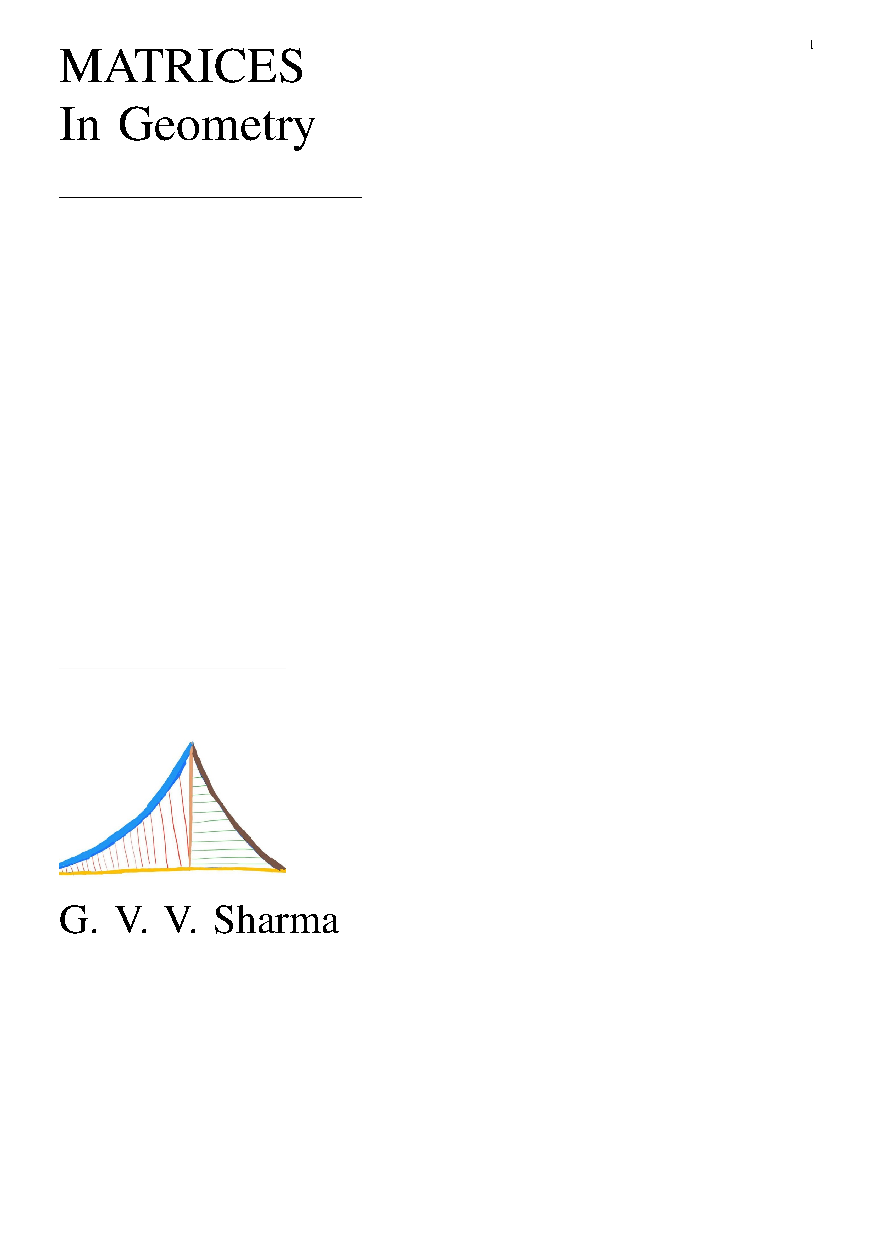
\includegraphics[width=0.75\columnwidth]{chapters/12/6/3/8/figs/main.png}
		\caption{}
		\label{fig:12/6/3/8}
  	\end{figure}
The equation of the conic can be represented as
\begin{align}
\vec{x}^{\top}\myvec{1&0\\0&0}\vec{x}+2\myvec{-2&\frac{-1}{2}}\vec{x}+4=0
\end{align}
So,
\begin{align}
\vec{V}=\myvec{1&0\\0&0},
\vec{u}^{\top}=\myvec{-2&\frac{-1}{2}},
f=4
\end{align}
The direction vector of the line passing through (2,0) and (4,4) is 
\begin{align}
\vec{m}=\myvec{1\\2}
\implies
\vec{n}=\myvec{2\\-1}.
\end{align}
The eigenvector corresponding to the zero eigenvalue is 
\begin{align}
\vec{p}_1=\myvec{0\\1},
\end{align}
In
\eqref{eq:conic_tangent_q_eigen},
\begin{align}
	\kappa=\frac{\myvec{0&1}\myvec{-2\\ \frac{-1}{2}}}{\myvec{0&1}\myvec{2\\-1}}
	=\frac{1}{2}
\end{align}
Substituting  $\kappa$,
from 
\eqref{eq:conic_tangent_q_eigen},
\begin{align}
	\myvec{\sbrak{\myvec{-2\\\frac{-1}{2}}+\frac{1}{2}\myvec{2\\-1}}^{\top} \\ \myvec{1&0\\0&0}}\vec{q} &= \myvec{-4 \\ \frac{1}{2}\myvec{2\\-1}-\myvec{-2\\\frac{-1}{2}}}\\
	\implies
	\myvec{-1&-1 \\ 1&0 \\ 0&0}\vec{q}&=\myvec{-4 \\ 3 \\ 0}
\end{align}
yielding
\begin{align}
\myvec{-1&-1 \\ 1&0}\vec{q} = \myvec{-4\\3}
\end{align}
The augmented matrix is 
\begin{align*}
  \myvec{
                -1&-1&\vrule&-4\\
	        1&0&\vrule&3}
  \xleftrightarrow[]{R_1 \leftarrow R_1+ 2R_2}
     \myvec{
	         1&-1&\vrule&2\\
	         1&0&\vrule&3}
      \\
 \xleftrightarrow[]{R_2 \leftarrow R_2 - R_1}
     \myvec{
	         1&-1&\vrule&2\\
	         0&1&\vrule&1}
 \xleftrightarrow[]{R_1 \leftarrow R_1 + R_2}
     \myvec{
	         1&0&\vrule&3\\
	         0&1&\vrule&1}
      \\ \implies \vec{q}=\myvec{3\\1}
\end{align*}
which is the desired 
point of contact.
See Fig. 
		\ref{fig:12/6/3/8}.

\item 
Find the equation of all lines having slope  -1 that are tangents to the curve
\begin{align}
y = \frac{1}{x-1}, x \neq 1
\label{chapters/12/6/3/10}
\end{align}
	\\
	\solution 
	\begin{figure}[H]
		\centering
 \includegraphics[width=0.75\columnwidth]{chapters/12/6/3/10/figs/conic1.pdf}
		\caption{}
		\label{fig:12/6/3/10}
  	\end{figure}
From the given information, 
\begin{align}
	\vec{V}
	=\myvec{
		0 & \frac{1}{2}\\\frac{1}{2}& 0\\
	},
\vec{u} = \myvec{
0 \\-\frac{1}{2}\\
},  f = -1, m=-1
	\label{eq:matrix-10-13-param}
\end{align}
From the above, the  normal vector is
\begin{align}
\vec{n}=\myvec{
-m \\ 1
	} = \myvec{1 \\ 1}
	\label{eq:matrix-10-13-param-n}
\end{align}
From 
\eqref{eq:conic_tangent_qk},
	the point(s) of contact are given by
\begin{align}
	\vec{q}&=\vec{V}^{-1}(k_i\vec{n}-\vec{u}) 
	\text{ where},\\
	k_i&=\pm \sqrt{\frac{f_0}{\vec{n}^{\top}\vec{V}^{-1}\vec{n}}}\\
	f_0&=f+\vec{u}^{\top}\vec{V}^{-1}\vec{u}
\end{align}
Substituting from 
	\eqref{eq:matrix-10-13-param-n}
	and
	\eqref{eq:matrix-10-13-param}
	in the above,
\begin{align}
\vec{q}=\myvec{0 \\-1}, \myvec{2 \\ 1}.
\end{align}
From 
  \eqref{eq:conic_tangent_final},
the equations of tangents are given by
\begin{align}
(\vec{V}\vec{q}+\vec{u})^{\top}\vec{x}+\vec{u}^{\top}\vec{q}+f=0
\end{align}
yielding
\begin{align}
	\myvec{1 & 1}\vec{x}+1&=0\\
\myvec{1 & 1}\vec{x}-3&=0\\
\end{align}
See 
		\figref{fig:12/6/3/10}.

\item 
Find the equation of all lines having slope 2 which are tangents to the curve 
\begin{align}
y=\frac{1}{x-3}, x\neq{3} 
\end{align}
\solution 
\label{chapters/12/6/3/11}
	\begin{figure}[H]
		\centering
 \includegraphics[width=0.75\columnwidth]{chapters/12/6/3/11/figs/con_fig.png}
		\caption{}
		\label{fig:12/6/3/11}
  	\end{figure}
From the given information
\begin{align}
	\vec{V}
	&=\myvec{
		0 &\frac{1}{2}\\\frac{1}{2} & 0\\
	},
\vec{u} = \myvec{
0 \\-\frac{3}{2}
},  f = -1, m=2
	\label{12/6/3/11/eq1}
	\\
	\implies
	\vec{n}&=\myvec{
-m \\ 1 
} = \myvec{-2 \\ 1}  \\
\label{12/6/3/11/eq2}
\end{align}
Hence, the given curve is a hyperbola.
%\raggedright
Substituting  numerical values, we obtain the condition in 
	\eqref{prop:conic-p-contact-nonparab-cond},
which implies that the line with slope 2 is not a tangent.  This can be verified from  
		\figref{fig:12/6/3/11}.

\item 
 Find points on the curve $\frac{x^2}{9}+\frac{y^2}{16}=1$ at which the tangents are 
 \begin{enumerate}
	 \item parallel to x-axis\\  
	 \item parallel to y-axis
 \end{enumerate}
 \solution 
\label{chapters/12/6/3/13}
	\begin{figure}[H]
		\centering
 \includegraphics[width=0.75\columnwidth]{chapters/12/6/3/13/figs/conic_1.pdf}
		\caption{}
		\label{fig:12/6/3/13}
  	\end{figure}
The parameters of the given conic are
\begin{align}
	\lambda_1&=16,\lambda_2=9 \\ \vec{V} &= \myvec{	\lambda_1& 0 \\
			          0 & \lambda_2}  
		    , \vec{u} = \myvec{0 \\0}, f = -144
		\label{eq:12/6/3/13/params}
	\end{align}
\begin{enumerate}
	\item The 
normal vector  in this case is
\begin{align}
		\vec{n_1}=\myvec{0\\1}
\end{align}
which can be used along with the parameters in 
		\eqref{eq:12/6/3/13/params}
		to obtain 
\begin{equation}
\vec{q_1}=\myvec{0\\4},
\vec{q_2}=\myvec{0\\-4}
\end{equation}
using 
\eqref{eq:conic_tangent_qk}.
\item Simlarly, 
	choosing
\begin{align}
	\vec{n_2}&=\myvec{1\\0},
	\\
	\vec{q_3}&=\myvec{3\\0},
	\vec{q_4}=\myvec{-3\\0}
\end{align}
\end{enumerate}
		See \figref{fig:12/6/3/13}.

\item 
Find the equation of the tangent line to the curve
\begin{align}
y=x^2-2x+7
\end{align}
\begin{enumerate}
    \item parallel to the line $2x-y+9=0$.
    \item perpendicular to the line $5y-15x=13$.
\end{enumerate}
\solution
\label{chapters/12/6/3/15}
	\begin{figure}[H]
		\centering
 \includegraphics[width=0.75\columnwidth]{chapters/12/6/3/15/figs/conic.png}
		\caption{}
		\label{fig:12/6/3/15}
  	\end{figure}
The parameters of the given conic are
\begin{align}
\vec{V} =\myvec{
	1 & 0\\
	0 & 0
	},
    \vec{u}=-\myvec{
	1 \\
	\frac{1}{2}
	},
    f=7
    \end{align}
\begin{enumerate}
	\item In this case,  the normal vector
		\begin{align}\vec{n}_1 = \myvec{2 \\ -1}\end{align}
			Since 
$\vec{V}$ is not invertible,  
		%Then given the normal vector \begin{align}\vec{n}\end{align}\, 
	the point of contact is given by 
\eqref{eq:conic_tangent_q_eigen} resulting in 
		%the matrix equation
\begin{align}
\myvec{\myvec{-1 \\ -\frac{1}{2}} + \frac{1}{2}\myvec{2 \\ -1}^{\top} \vspace{0.3cm}\\ \myvec{
	1 & 0\\
	0 & 0\\
	}} \vec{q}_1 = \myvec{-7 \vspace{0.3cm}\\ \frac{1}{2}\myvec{2 \\ -1} - \myvec{-1 \\ -\frac{1}{2}}}
\end{align}
By solving the above equation, we can get the point of contact as
    \begin{align}
  \vec{q}_1=\myvec{
	2 \\
	7 \\
	}
\end{align}
The 
tangent equation is then obtained as
\begin{align}
      \vec{n}_1^{\top}(\vec{x}-\vec{q}_1) = 0
  \\
	\implies  \myvec{2 & -1}\vec{x}+3 = 0
\end{align}
\item 
In this case, 
		\begin{align}\vec{n}_2 = \myvec{1 \\ 3} \end{align}
resulting in 
\begin{align}
\myvec{\myvec{-1 \\ -\frac{1}{2}} + -\frac{1}{6}\myvec{1 \\ 3}^{\top} \vspace{0.3cm}\\ \myvec{
	1 & 0\\
	0 & 0\\
	}} \vec{q}_2 = \myvec{-7 \vspace{0.3cm}\\ -\frac{1}{6}\myvec{1 \\ 3} - \myvec{-1 \\ -\frac{1}{2}}}
\end{align}
    \begin{align}
	    \text{or, }  \vec{q}_2=\myvec{
	\frac{5}{6}
\\
	\frac{217}{36}
	}
\end{align}
The tangent equation is
\begin{align}
      \vec{n}_2^{\top}(\vec{x}-\vec{q}_2) = 0
      \\
	\text{or, }    \myvec{1 & 3}\vec{x}= \frac{227}{12}
\end{align}
\end{enumerate}
		See \figref{fig:12/6/3/15}.

\item 
Find the equation of the tangent to the curve 
\begin{align}
	y = \sqrt{3x-2}
\end{align}
which is parallel to the line
\begin{align}
	4x-2y+5 = 0
\end{align}
\solution 
\label{chapters/12/6/3/25}
The parameters for the given conic are
\begin{align}
	\label{12/6/3/25eq:V_matrix}
	\vec{V} &= \myvec{0 & 0\\0 & 1},
	\\
	\label{12/6/3/25eq:u_vector}
	\vec{u} &= \myvec{-3/2\\0},
	\\
	\label{12/6/3/25eq:f_value}
	f &= 2
	%\\
\end{align}
which represent a parabola. 
Following the approach in 
\probref{chapters/12/6/3/15},
   \begin{align}
     \vec{p_1} = \myvec{1\\0},\
     \vec{n} = \myvec{-2\\1},
    \end{align}
yielding the matrix equation
\begin{align}
	\label{12/6/3/25eq:vertex_system}
	\myvec{-3&0\\0& 0\\0& 1}\vec{q} = \myvec{-41/16\\0 \\3/4}\\
\end{align}
The augmented matrix for \eqref{12/6/3/25eq:vertex_system} can be expressed as
\begin{align*}
	%\label{12/6/3/25eq:vertex_solv1}
	%\myvec{-3&0&\vrule&2\\0&0&\vrule&0\\0&1&\vrule&0}\\ 	
	%\label{12/6/3/25eq:vertex_solv2}
	\xleftrightarrow[]{R_2 \leftrightarrow R_3}\myvec{-3&0&\vrule&-41/16\\0&1&\vrule&0\\0&0&\vrule&3/4}
	\xleftrightarrow[]{-\frac{R_1}{-3} \leftarrow R_2}\myvec{1&0&\vrule&41/48\\0&1&\vrule&0\\0&0&\vrule&3/4}\\
	\implies\vec{q} = \myvec{\frac{41}{48}\\\frac{3}{4}}
\end{align*}
The equation of tangent is then obtained as
\begin{align}
	\myvec{-2 & 1}\vec{x} +\frac{23}{24} = 0 
\end{align}
See  
		\figref{fig:12/6/3/25}.
	\begin{figure}[H]
		\centering
 \includegraphics[width=0.75\columnwidth]{chapters/12/6/3/25/figs/conic.pdf}
		\caption{}
		\label{fig:12/6/3/25}
  	\end{figure}

\item 
Find the point at which the line $y = x + 1$ is a tangent to the curve $y^2 = 4x$.
\\
\solution 
\label{chapters/12/6/3/27}
	\begin{figure}[H]
		\centering
 \includegraphics[width=0.75\columnwidth]{chapters/12/6/3/27/figs/conicfig.png}
		\caption{}
		\label{fig:12/6/3/27}
  	\end{figure}
The parameters of the conic are
\begin{align}
 \vec{V} = \myvec{0&0\\0&1},  \vec{u} = \myvec{-2&0}, f = 0 
\end{align}
Following the approach in Problem 
\ref{chapters/12/6/3/15},
since
\begin{align}
	\vec{n} = \myvec{1 \\ -1}
\end{align}
we obtain
\begin{align}
	\vec{q} = \myvec{1 \\ 2}
\end{align}
See 
		\figref{fig:12/6/3/27}.


    \item The point on the curve 
\label{chapters/12/6/5/27}
    \begin{align}
        x^2 = 2y
        \label{eq:chapters/12/6/5/27/curve}
    \end{align}
    which is nearest to the point 
    $\vec{P} = \myvec{0\\5}$ is
    \begin{enumerate}
        \item $\myvec{2\sqrt{2}\\4}$
        \item $\myvec{2\sqrt{2}\\0}$
        \item $\myvec{0\\0}$
        \item $\myvec{2\\2}$
    \end{enumerate}
    \solution 
		We rewrite the conic \eqref{eq:chapters/12/6/5/27/curve} in matrix form.
    \begin{align}
        \vec{x}^\top\myvec{1&0\\0&0}\vec{x} + 2\myvec{0&-1}\vec{x} = 0
        \label{eq:chapters/12/6/5/27/curve-mtx}
    \end{align}
    Comparing with the general equation of the conic,
    \begin{align}
        \vec{V}_0 = \myvec{1&0\\0&0},\
        \vec{u}_0 = \myvec{0\\-1},\ 
        f_0 = 0 
    \end{align}
    Therefore, the equation of the normal where $\vec{q}$ is the point of contact 
    and 
\begin{align}
    \vec{R} \triangleq \myvec{0&-1\\1&0} 
\end{align}
is
    \begin{align}
	    \brak{\vec{V}_0\vec{q}+\vec{u}_0}^\top\vec{R}\brak{\myvec{0\\5}-\vec{q}} &= 0
        \label{eq:chapters/12/6/5/27/normal}
    \end{align}
    Substituting appropriate values and simplifying, we get 
    \begin{align}
	    \vec{q}^\top\myvec{0&1\\0&0}\vec{q} + 2\myvec{-2 & 0}\vec{q}= 0
        \label{eq:chapters/12/6/5/27/q-eqn}
    \end{align}
    which can be expressed as 
    \begin{multline}
	    \frac{1}{2}\lcbrak{
		    \vec{q}^\top\myvec{0&1\\0&0}\vec{q} + 2\myvec{-2 & 0}\vec{q}}
	\\
	    +
	    \rcbrak{
		    \vec{q}^\top\myvec{0&1\\0&0}^\top\vec{q} + 2\myvec{-2 & 0}\vec{q}}= 0
    \end{multline}
    yielding
    \begin{align}
	    \vec{q}^\top\myvec{0&\frac{1}{2}\\\frac{1}{2}&0}\vec{q} + 2\myvec{-2 &0}\vec{q} = 0
        \label{eq:chapters/12/6/5/27/q-affine}
    \end{align}
        \eqref{eq:chapters/12/6/5/27/q-affine}
	also looks like a conic with parameters
    \begin{align}
        \vec{V} = \myvec{1&0\\0&0},\
        \vec{u} = \myvec{0\\-1},\ 
        f = 0 
    \end{align}
The eigenparameters of $\vec{V}$ are
    \begin{align}
        \label{eq:chapters/12/6/5/27/PD}
        \vec{P} = \myvec{1&1\\1&-1},\ \vec{D} = \myvec{1&0\\0&-1}
    \end{align}
    Applying the affine transformation
    \begin{align}
        \label{eq:chapters/12/6/5/27/affine}
        \vec{q} &= \vec{Py} + \vec{c} \\
        \vec{c} &= -\vec{V}^{-1}\vec{u} 
 =\myvec{0\\4} \\
        f_0 &= \vec{u}^\top\vec{V}^{-1}\vec{u} - f 
            =  0
    \end{align}
$\because \det{V} = -\frac{1}{4} \neq 0$, 
	  using \eqref{eq:pair-cond},
        \eqref{eq:chapters/12/6/5/27/q-affine}
 represents a pair of straight lines.
      From \eqref{eq:pair-conic},
        \eqref{eq:chapters/12/6/5/27/PD},
	\eqref{eq:incircle-disc-v}
	and 
	\eqref{eq:incircle-disc-v-lam},
    \begin{align}
%        y_1^2-y_2^2 &= 0 \\
%        \implies y_1 &= \pm y_2 \\
%        \implies \vec{y} &= \myvec{a\\\pm a},\ a \in \mathbb{R}
\vec{y} = \kappa\myvec{1\\\pm 1}.
        \label{eq:chapters/12/6/5/27/y-sol}
    \end{align}
    Hence, using 
        \eqref{eq:chapters/12/6/5/27/affine},
    \begin{align}
        \vec{q} 
                = \myvec{0\\4}+\kappa\myvec{1\\\pm 1},
%                &= \myvec{a\pm a\\a\mp a+4} \\
        \label{eq:chapters/12/6/5/27/x-case}
    \end{align}
which, upon substituting in 
        \eqref{eq:chapters/12/6/5/27/curve-mtx}
	and solving for $\kappa$ yields
\begin{align}
	\kappa = \pm \sqrt{2}, -2.
\end{align}
 Thus, the points of contact are
    \begin{align}
        \vec{q}  = \cbrak{\myvec{\pm 2\sqrt{2}\\4},\myvec{0\\0}}
        \label{eq:chapters/12/6/5/27/poc-ans}
    \end{align}
    The nearest point out of these three candidates for $\vec{q}$ is
    $\myvec{\pm2\sqrt{2}\\4}$. 
See \figref{fig:chapters/12/6/5/27/normal}.
\begin{figure}[H]
        \centering
        \includegraphics[width=0.75\columnwidth]{chapters/12/6/5/27/figs/normal.png}
        \caption{}
        \label{fig:chapters/12/6/5/27/normal}
    \end{figure}

\item 
Find the equation of the normal to curve $x^2 = 4y$ which passes through the point
(1, 2).
\\
\solution 
\label{chapters/12/6/6/4}
	\begin{figure}[H]
		\centering
 \includegraphics[width=0.75\columnwidth]{chapters/12/6/6/4/figs/conics.png}
		\caption{}
		\label{fig:12/6/6/4}
  	\end{figure}
The conic parameters are
\begin{align}
	\vec{V} = \myvec{1 & 0\\0 & 0},
	\vec{u} = \myvec{0\\-2},
	f &= 0
	%\\
\end{align}
Choosing the direction and normal vectors as
\begin{align}
	\vec{m} = \myvec{1 \\ m}, \
	\vec{n} = \myvec{-m \\ 1}, 
\end{align}
and substituting these values in
	\eqref{eq:point_of_tangency-m},
% \eqref{eq:normal_solution}, 
 we obtain
\begin{align}
m = 1
\end{align}
as the only real solution.  Thus, 
\begin{align}
%\vec{n} = \myvec{1 \\ 1},
	\vec{m} = \myvec{1 \\ 1}, 
%    \mu = -1
\end{align}
and 
	the equation of the normal is then obtained as
\begin{align}
	\vec{m}^{\top}\brak{\vec{x}-\vec{h}} &= 0
	\\
	\implies
\myvec{
1 & 1
}
		\vec{x}
	&=
\myvec{
1 & 1
}
	\myvec{1 \\2 }
	\\
	&= 3
\end{align}
		See \figref{fig:12/6/6/4}.

\item 
 The line $y=mx+1$ is a tangent to the curve $y^2 = 4x$, find the value of $m$. 
 \\
 \solution 
\label{chapters/12/6/6/21}
	\begin{figure}[H]
		\centering
 \includegraphics[width=0.75\columnwidth]{chapters/12/6/6/21/figs/im.pdf}
		\caption{}
		\label{fig:12/6/6/21}
  	\end{figure}
The parameters for the given conic are
\begin{align}
    \vec{V} = \myvec{0&0\\0&1}, \vec{u} = \myvec{-2\\0}, f = 0
		\label{eq:12/6/6/21/param}
\end{align}
The given tangent can be expressed in parametric form as
\begin{align}
		\label{eq:12/6/6/21/tangent}
\vec{x} = \vec{e}_2 + \mu\vec{m}
\end{align}
Substituting from 
		\eqref{eq:12/6/6/21/tangent}
		and
		\eqref{eq:12/6/6/21/param}
		in 
	  \eqref{eq:h-tangents-cond}
and solving, we obtain 
\begin{align}
	m = 1.
\end{align}
		See \figref{fig:12/6/6/21}.

\item 
\label{chapters/12/6/6/22}
Find the normal at the point (1,1) on the curve 
\begin{align}
2y+x^2=3
\end{align}
\solution
Use
  \eqref{eq:conic_tangent_mq}
  with 
\begin{align}
	\vec{m} = \myvec{1 \\m}
\end{align}

 \item If the line $y=\sqrt{3}x+K$ touches the parabola $x^2=16y,$ then find the value of $K$.
\item If the line $y=mx+1$ is tangent to the parabola $y^2=4x$ then find the value of $m$.
\item Find the condition that the curves $2x=y^2$ and $2xy=k$ intersect orthogonally.
\item Prove that the curves $xy=4$ and $x^2+y^2=8$ touch each other.
\item Find the angle of intersection of the curves $y=4-x^2$ and $y=x^2$.
\item Prove that the curves $y^2=4x$ and $x^2+y^2-6x+1=0$ touch each each other at the point (1,2).
\item Find the equation of the normal lines to the curve $3x^2-y^2=8$ which are parallel to the line $x+3y=4$.
 \item The equation of the normal to the curve $3x^2-y^2 =8$ which is parallel to the line $x+3y=8$ is
 \begin{enumerate}
 \item $3x-y=8$
 \item $3x+y+8=0$
 \item $x+3y+8=0$
 \item $x+3y=0$
 \end{enumerate}
\item The equation of the tangent to the curve $(1+y^2) =2-x$, where it crosses the x-axis is 
\begin{enumerate}
\item $x+5y=2$
\item $x-5y=2$
\item $5x-y=2$
\item $5x+y=2$
\end{enumerate}
\end{enumerate}
State whether the statements are True or False 
\begin{enumerate}[label=\thesection.\arabic*,ref=\thesection.\theenumi,resume*]
\item The line $lx+my+n=0$ will touch the parabola $y^2=4 ax$ if $ln =am^2$,
\item The line $2x+3y=12$ touches the ellipse $\frac{x^2}{9}+\frac{y^2}{4}=2$ at the point (3,2).
\end{enumerate}
